\documentclass{article}
\usepackage{graphicx}
\usepackage{listings}
\usepackage{xcolor}
\usepackage{hyperref}
\usepackage{amsmath}
\usepackage{geometry}
\usepackage{float}
\geometry{a4paper, margin=1in}

\definecolor{codegreen}{rgb}{0,0.6,0}
\definecolor{codegray}{rgb}{0.5,0.5,0.5}
\definecolor{codepurple}{rgb}{0.58,0,0.82}
\definecolor{backcolour}{rgb}{0.95,0.95,0.92}

\lstdefinestyle{mystyle}{
    backgroundcolor=\color{backcolour},   
    commentstyle=\color{codegreen},
    keywordstyle=\color{magenta},
    numberstyle=\tiny\color{codegray},
    stringstyle=\color{codepurple},
    basicstyle=\ttfamily\footnotesize,
    breakatwhitespace=false,         
    breaklines=true,                 
    captionpos=b,                    
    keepspaces=true,                 
    numbers=left,                    
    numbersep=5pt,                  
    showspaces=false,                
    showstringspaces=false,
    showtabs=false,                  
    tabsize=2
}

\lstset{style=mystyle}

\title{Scientific Calculator using AVR GCC}
\author{MANOGNYA K - EE24BTECH11037}
\date{\today}

\begin{document}

\maketitle

\begin{abstract}
This report documents the design and implementation of a scientific calculator using AVR microcontrollers programmed with AVR GCC. The calculator features a 16x2 LCD display, 10-digit input buttons, and multiple operation modes including basic arithmetic, trigonometric functions, logarithmic functions, and more. The implementation includes custom numerical approximations for mathematical functions using the Forward Euler method.
\end{abstract}

\tableofcontents

\section{Introduction}
The AVR-based scientific calculator is designed to provide a wide range of mathematical operations while maintaining a simple hardware interface. The project demonstrates the integration of multiple components including:

\begin{itemize}
    \item AVR microcontroller (ATmega328P)
    \item 16x2 LCD display
    \item Push buttons for Input 
    \item Custom mathematical function implementations
    \item Multiple operation modes
\end{itemize}

\section{Hardware Design}
The calculator uses the following hardware components:

\subsection{Microcontroller}
The project is designed for AVR microcontrollers (ATmega328P) running at 16MHz clock frequency.

\subsection{LCD Interface}
The 16x2 LCD is connected in 4-bit mode to conserve I/O pins:
\begin{itemize}
    \item VSS - GND
    \item VDD - 5V
    \item $V_0$ - middle pin of potentiometer 
    \item RS (Register Select) - 12
    \item RW (Read/Write) - GND
    \item EN (Enable) - 11
    \item Data pins D4-D7 - PD5-PD2
    \item A(Backlight) - 5V
    \item K(Backlight) - GND 
\end{itemize}
The reference diagram for the LCD pins and their functions is shown below : \\
\begin{figure}[htbp]
    \centering
    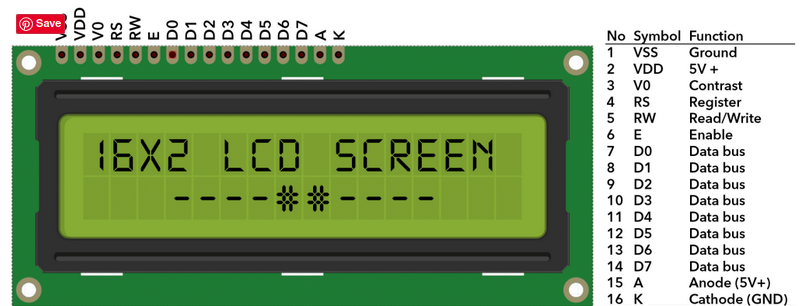
\includegraphics[width=0.8\textwidth]{Screenshot from 2025-03-24 21-25-56.png} % Replace with your image filename
    \caption{16x2 LCD for reference}
    \label{fig:example}
\end{figure}
\subsection{Input Buttons}
\begin{itemize}
    \item 10 digit buttons (0-9) connected to pins 6-10 and 14-18 (A0-A4)
    \item Shift button (A5) for accessing secondary functions
    \item Extra mode button (digital pin 13) for advanced functions
    \item Other terminal of the buttons is grounded
\end{itemize}
$\bullet$ The table for the buttons is shown below; \\
\begin{table}[h]
\centering
\begin{tabular}{|l|l|l|}
\hline
\textbf{Button} & \textbf{Right Toggle} & \textbf{Left Toggle} \\ \hline
     2 &  + & $sin^{-1}$ \\ \hline
     3 &  - & $cos^{-1}$ \\ \hline
     4 &  * & $tan^{-1}$ \\ \hline
     5 &  / & $log_{10}$ \\ \hline
     6 & = & ln \\ \hline
     7 & backspace & \\ \hline
     8 & sin &  \\ \hline
     9 & cos & \\ \hline
     10 & $e^x$ & \\ \hline
     11 & $\sqrt{}$ & \\ \hline 
\end{tabular}
\end{table}
\subsection{Potentiometer}
\begin{itemize}
    \item The middle wire is connected to $V_0$ via 220$\Omega$ resistor
    \item One end is grounded and other is connected to $5V$
\end{itemize}
$\bullet$ The overall circuit connections are summarized in the table figue; 
\begin{table}[h]
\centering
\caption{Connection Details}
\begin{tabular}{|l|l|}
\hline
\textbf{LCD} & \textbf{Connection} \\ \hline
1 & GND \\ \hline
2 & 5v \\ \hline
3 & potentiometer (middle) \\ \hline
4 & 12 \\ \hline
5 & gnd \\ \hline
6 & 11 \\ \hline
7 & unused \\ \hline
8 & unused \\ \hline
9 & unused \\ \hline
10 & unused \\ \hline
11 & 5 \\ \hline
12 & 4 \\ \hline
13 & 3 \\ \hline
14 & 2 \\ \hline
15 & 5v \\ \hline
16 & gND \\ \hline
\end{tabular}
\quad
\begin{tabular}{|l|l|}
\hline
\textbf{Buttons} & \textbf{Connection} \\ \hline
1 & 13 \\ \hline
2 & 6 \\ \hline
3 & 7 \\ \hline
4 & 8 \\ \hline
5 & 9 \\ \hline
6 & 10 \\ \hline
7 & A0 \\ \hline
8 & A1 \\ \hline
9 & A2 \\ \hline
10 & A3 \\ \hline
11 & A4 \\ \hline
12 & A5 \\ \hline
\end{tabular}
\end{table}\\
$\bullet$ The below is the circuit that I have set up;
\begin{figure}[H]
    \centering
    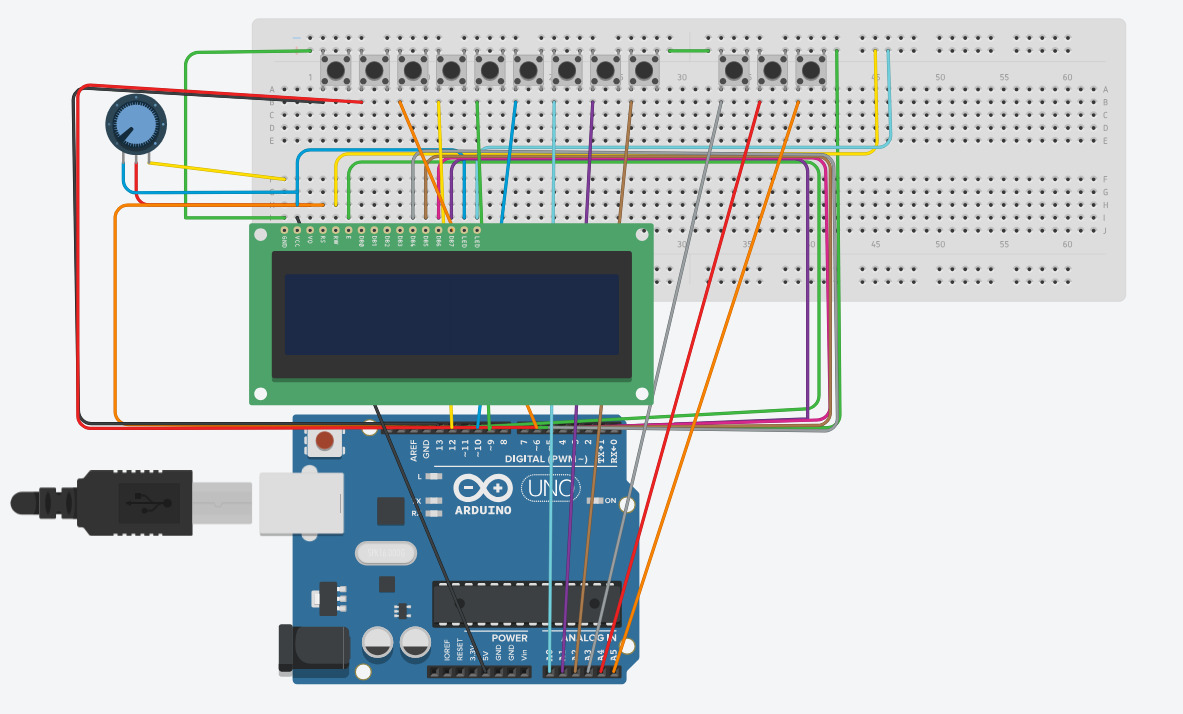
\includegraphics[width=0.8\textwidth]{WhatsApp Image 2025-03-24 at 22.39.09.jpeg} % Replace with your image filename
    \caption{Circuit Setup}
    \label{fig:example}
\end{figure}
\section{Software Architecture}
The software is structured into several key components:

\subsection{Main Program Flow}
The program follows the standard Arduino-style structure with \texttt{setup()} and \texttt{loop()} functions:
\begin{itemize}
    \item \texttt{setup()} initializes the LCD and button inputs
    \item \texttt{loop()} continuously checks button states and processes input
\end{itemize}

\subsection{Input Processing}
The calculator implements three operation modes:
\begin{itemize}
    \item Normal mode (digits 0-9)
    \item Shift mode (arithmetic operations and basic functions)
    \item Extra mode (advanced mathematical functions)
\end{itemize}

\subsection{Display Management}
The LCD display shows:
\begin{itemize}
    \item Current input expression (up to 32 characters across two lines)
    \item Calculation results with 3 decimal places precision
\end{itemize}

\section{Mathematical Function Implementations}
The calculator implements several mathematical functions using numerical approximations:

\subsection{Trigonometric Functions}
The sine and cosine functions are implemented using the Forward Euler method on the coupled ordinary differential equations:
\begin{align*}
    \frac{dy}{dx} &= z \quad \text{(where } y = \sin(x)\text{)} \\
    \frac{dz}{dx} &= -y \quad \text{(where } z = \cos(x)\text{)}
\end{align*}

\subsection{Exponential Function}
The exponential function uses Forward Euler on:
\[ \frac{dy}{dx} = y \]

\subsection{Square Root}
Implemented using Newton's method:
\[ x_{n+1} = \frac{1}{2}\left(x_n + \frac{a}{x_n}\right) \]

\subsection{Logarithmic Functions}
The natural logarithm uses:
\[ \frac{dy}{dx} = \frac{1}{x} \]
with initial condition \( y(1) = 0 \).

\section{Code Structure}
The main components of the code are:

\subsection{LCD Interface}
\begin{lstlisting}[language=C]
void LCD_Command(unsigned char cmnd);
void LCD_Char(unsigned char data);
void LCD_Init();
void LCD_String(const char* str);
void LCD_Clear();
\end{lstlisting}

\subsection{Button Handling}
\begin{lstlisting}[language=C]
void pinMode(int pin, int mode);
int digitalRead(int pin);
void handleSpecial(char op);
\end{lstlisting}

\subsection{Mathematical Functions}
\begin{lstlisting}[language=C]
float mySin(float x);
float myCos(float x);
float myExp(float x);
float mySqrt(float x);
float myAsin(float x);
float myAcos(float x);
float myAtan(float x);
float myLn(float x);
float myLog10(float x);
\end{lstlisting}

\subsection{Expression Evaluation}
\begin{lstlisting}[language=C]
float evaluateFullExpression(const char* expr);
float evaluateExpression(const char* expr);
\end{lstlisting}

\section{Challenges and Solutions}
\subsection{Numerical Approximation Accuracy}
The Forward Euler method provides reasonable accuracy for the calculator's purposes, though more advanced methods (like Runge-Kutta) could improve precision.

\subsection{Button Debouncing}
Software debouncing is implemented with a 50ms delay after detecting a button press.

\subsection{Memory Constraints}
The AVR's limited RAM requires careful management of string buffers and intermediate calculation results.

\section{Conclusion}
The AVR-based scientific calculator successfully demonstrates:
\begin{itemize}
    \item Integration of multiple hardware components
    \item Implementation of complex mathematical functions on limited hardware
    \item User interface design for embedded systems
    \item Numerical methods for function approximation
\end{itemize}

Future improvements could include:
\begin{itemize}
    \item Implementation of operator precedence
    \item Additional mathematical functions
    \item Hardware PCB design for a standalone device
    \item Power management for battery operation
\end{itemize}

\end{document}r
